\newpage
\section{Introduction}
\label{sec:introduction}

% state the learning objective 
The objective of this laboratory assignment is to study a circuit containing an Independent AC Voltage Souce, $V_s(t)$, a Voltage Controlled Current Source, $I_d$, a Current Controlled Voltage Source, $V_d$, a Capacitor $C$, and seven resistors, $R_1$ to $R_7$. The circuit that we were first presented with is displayed in Figure \ref{fig:circ}, with some added current directions to ease the process of finding equations in our Analysis section. As we make modifications to the circuit along the report to suit our needs, the circuit used for those will also be displayed.

\begin{figure}[h] \centering
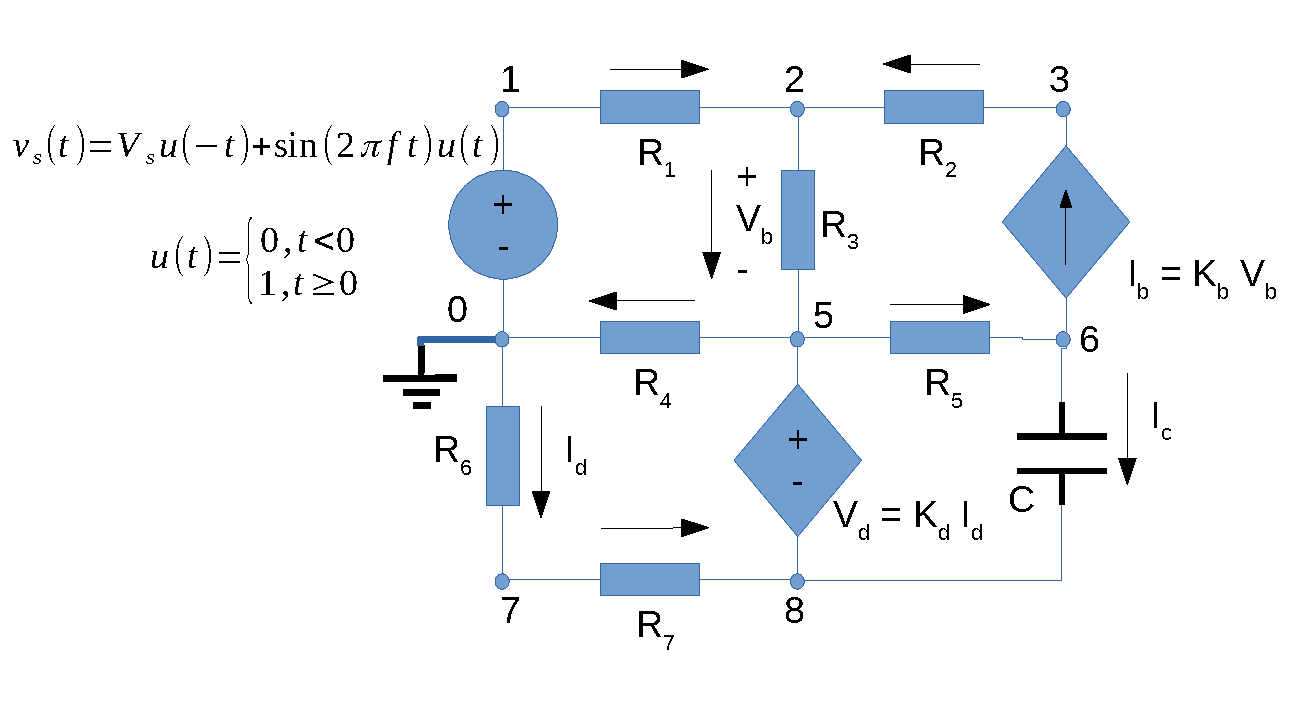
\includegraphics[width=0.6\linewidth]{t2-original.pdf}
\caption{The original circuit, with some current directions added.}
\label{fig1}
\end{figure}

In Section~\ref{sec:analysis}, a theoretical analysis of the circuit is
presented, including the study of what happens for $t<0$, finding the the equivalent resistor as seen from the capacitor
terminals, the natural and forced solutions of the circuit in $t>0$, as well as frequency analysis.

In Section~\ref{sec:simulation}, the circuit is analysed by
simulation using the \textit{software Ngspice}, ultimately, studying the same as in the Theoretical Analysis section.
The results in each Analsysis are compared NOVA SECÇÃO??????????????????????????????
The conclusions of this study are outlined in
Section~\ref{sec:conclusion}.
